\chapter{Comandos básicos}
Al inicio la terminal puede ser algo intimidante pero la terminal es tu amigo, y una
ves que aprendas a usarla dejaras de usar el mouse, bueno lo usaras muy poco.
A día de hoy la terminal tiene tanta personalización que he dejado de usar el mouse y
solo lo hago en muy pocos casos.
\\
Apretar Crtl + Alt + T para abrir la consola o terminal si no funciona puedes entra a tu
buscador de linux y buscar la terminal(Gnome) o también se suele llamar konsole(kde).

\begin{figure}[h]
	\centering

\includegraphics[width=1\textwidth]{image/chapter_01/terminal.png}
	\caption{Busqueda terminal linux.}
	\label{figura1}
\end{figure}

Deberías abrir tu terminal algo así, como mi terminal esta personalizada seguro tiene colores distintos a la tuya.
\begin{figure}[h]
	\centering
	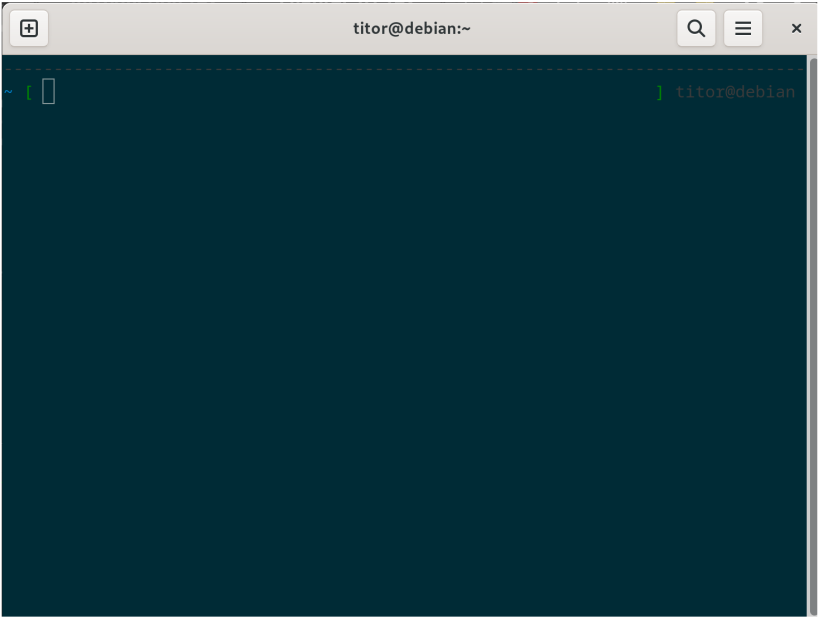
\includegraphics[width=0.7\textwidth]{image/chapter_01/konsole.png}
	\caption{Consola linux.}
	\label{figura1}
\end{figure}


\section{Los 10 comandos que usaras toda tu vida}
\begin{enumerate}
  \item \textbf{whoami}, who am I, El primer comando que aprenderemos es a saber quien soy yo(whoami)
\begin{lstlisting}[language=bash]
whoami
output : titor
  \end{lstlisting}
  Este comando nos indica el usuario que somos, en mi caso mi usuario se llama titor
  y todos los comandos que ejecute se realizara bajo este usuario.
  \item pwd, print working directory Comando para saber donde estoy parado.
  \begin{lstlisting}[language=bash]
pwd
output : / home / titor
  \end{lstlisting}
Este comando nos indica el lugar donde estamos osea en que directorio estamos trabajando la salida sera el la dirección en este caso el home es como el escritorio
en windows.
\item \textbf{ls} list, Comando para listar los archivos y directorios del lugar donde estamos
parados
Deberías recibir una vista similar con todos los archivos y directorios que tengas.

  \begin{lstlisting}[language=bash]
ls
  \end{lstlisting}

	\begin{figure}[h]
		\centering
	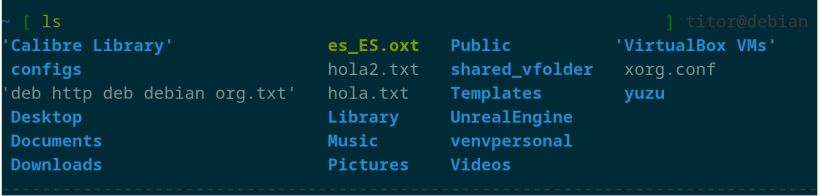
\includegraphics[width=1\textwidth]{image/chapter_01/ls.png}
		\caption{Resultado comando ls.}
		\label{figura1}
	\end{figure}


    Este comando también tiene \textbf{-banderas} que nos ayudan a ver información adicional
  de lo que vemos por ejemplo
 \begin{enumerate}
   \item \textbf{ls -a} Para ver archivos ocultos, los archivos ocultos llevan un . por delante
 \newpage
    \item \textbf{ls -l} Nos da información mas detallada, que significa


\begin{lstlisting}[language=bash]
ls -l
\end{lstlisting}
\begin{figure}[h]
	\centering
	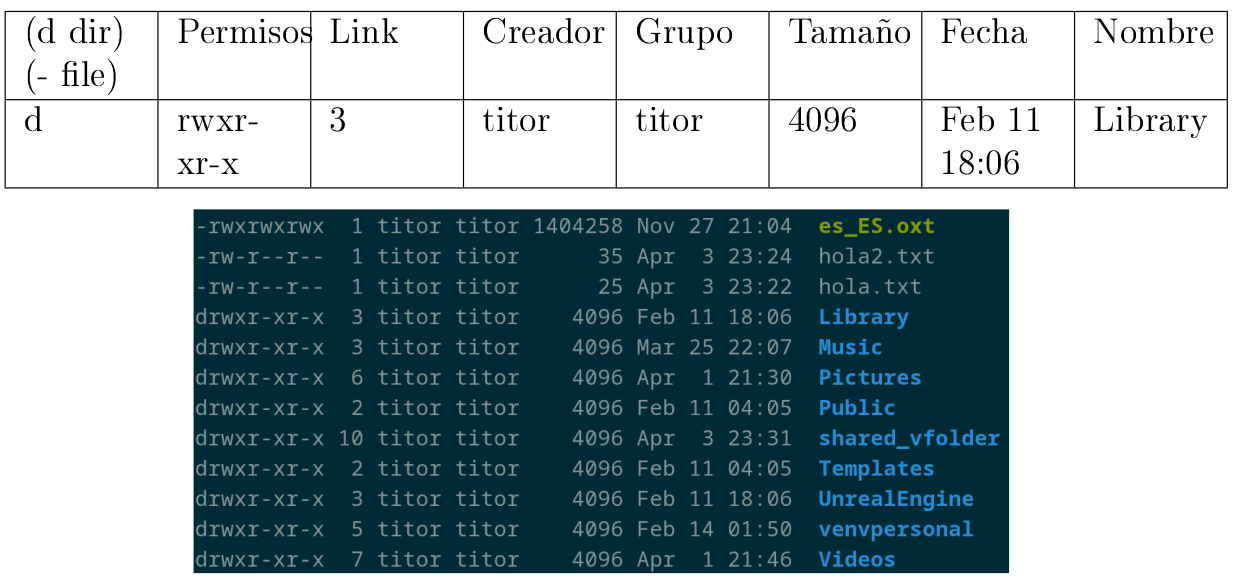
\includegraphics[width=1\textwidth]{image/chapter_01/lsalh.png}
	\caption{Resultado comando ls -l.}
	\label{figuralsl}
\end{figure}

\item \textbf{ls -alh} Mi favorito, (a) para ver archivos ocultos,(l) para lista detallada, (h)
para que a diferencia del anterior la columna tamaño sea mas entendible lleva
una K para Kbytes una M para mega bites G giga bytes.
\\
  
\begin{lstlisting}[language=bash]
ls -alh
\end{lstlisting}
	\begin{figure}[h]
	\centering
	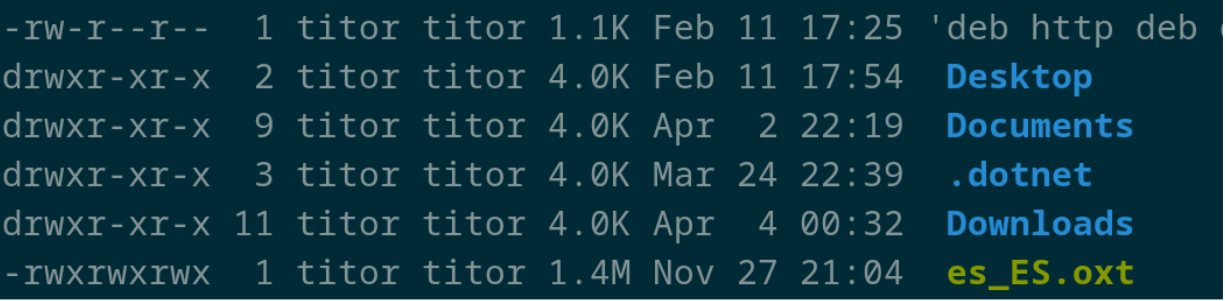
\includegraphics[width=1\textwidth]{image/chapter_01/lslah.png}	
	\caption{Resultado comando ls -alh.}
	\label{figura1}
\end{figure}

\end{enumerate} 
\item \textbf{cd} change directory, Comando para cambiar de directorio, entrar y salir de directorios.\\
Por ejemplo el comando ls para listar los archivos y directorios podría moverme a
ese directorio usando cd <nombre del directorio>

\begin{lstlisting}[language=bash]
cd Documents
\end{lstlisting}
Entraríamos a la carpeta Documents y si escribimos pwd nos debería decir que ahora estamos en /home/titor/Documents
\begin{lstlisting}[language=bash]
cd Documents
\end{lstlisting}
También podemos ingresar cada ves mas adentro acoplando el nombre de la carpeta seguido del símbolo / ejemplo:
\begin{lstlisting}[language=bash]
cd Documents / carpeta_1 / carpeta_2 / capeta_3
\end{lstlisting}
\item \textbf{touch}, Comando que nos permite crear un archivo en el lugar donde estamos parados tenemos que acompañar touch seguido del nombre del archivo que va a crearse, o si el archivo ya existe le da un toque lo cual modifica la ultima fecha de modificación puedes verificarlo con el comando ls -lh
\begin{lstlisting}[language=bash]
touch nombre_archivo . txt
\end{lstlisting}
Podemos crear varios archivos Creara estos tres archivos:
\begin{lstlisting}[language=bash]
touch nombre_archivo1.txt nombre_archivo2.py nombre_archivo3...
\end{lstlisting}
\item \textbf{mkdir}, Comando que nos permite crear directorios en lugar donde estamos parados tenemos que acompañar mkdir seguido del nombre del directorio que va a crearse
\begin{lstlisting}[language=bash]
mkdir nombre_folder
\end{lstlisting}
Creara esos tres folders o también llamadas carpetas
\begin{lstlisting}[language=bash]
mkdir nombre_folder1 nombre_folder2 nombre_folder3
\end{lstlisting}
Ahora podemos crear un árbol de directorio con subfolders agregando la bandera
-p y siguiendo el siguiente formato
\begin{lstlisting}[language=bash]
mkdir -p folder_padre/{hijo1, hijo2/{nieto1, nieto2}, hijo3}
\end{lstlisting}
\item \textbf{rm} remove, Comando para eliminar podemos eliminar archivos con rm nombre\_archivo o podemos eliminar carpetas agregando la bandera -r, \textbf{rm -r} nombre\_folder
\begin{lstlisting}[language=bash]
rm nombre_archivo.txt
rm -r folder_padre
\end{lstlisting}
\item \textbf{popd} retroceder, Comando retroceder al anterior lugar, por ejemplo si usamos cd
para ir del punto a al b cd foler1/folder2/folder3/foler4 usando popd volvemos al punto a.
\begin{lstlisting}[language=bash]
pwd
output: /home/titor/
cd foler1/folder2/folder3/foler4
pwd
output: /home/titor/foler1/folder2/folder3/foler4
popd
pwd
output: /home/titor/
\end{lstlisting}
Volvemos a estar en lugar anterior.
\item \textbf{clear}  Limpiamos la consola, también se puede usar \textbf{Ctrl+l} y limpiara la  consola sin necesidad de ejecutar ningún comando.
\begin{lstlisting}[language=bash]
clear
\end{lstlisting}
\newpage
\item \textbf{cat} Comando para imprimir y ver el contenido de un archivo en la consola sin tener que entrar al archivo.
\begin{lstlisting}[language=bash]
cat nombre_archivo.txt
\end{lstlisting}

\begin{figure}[h]
	\centering
  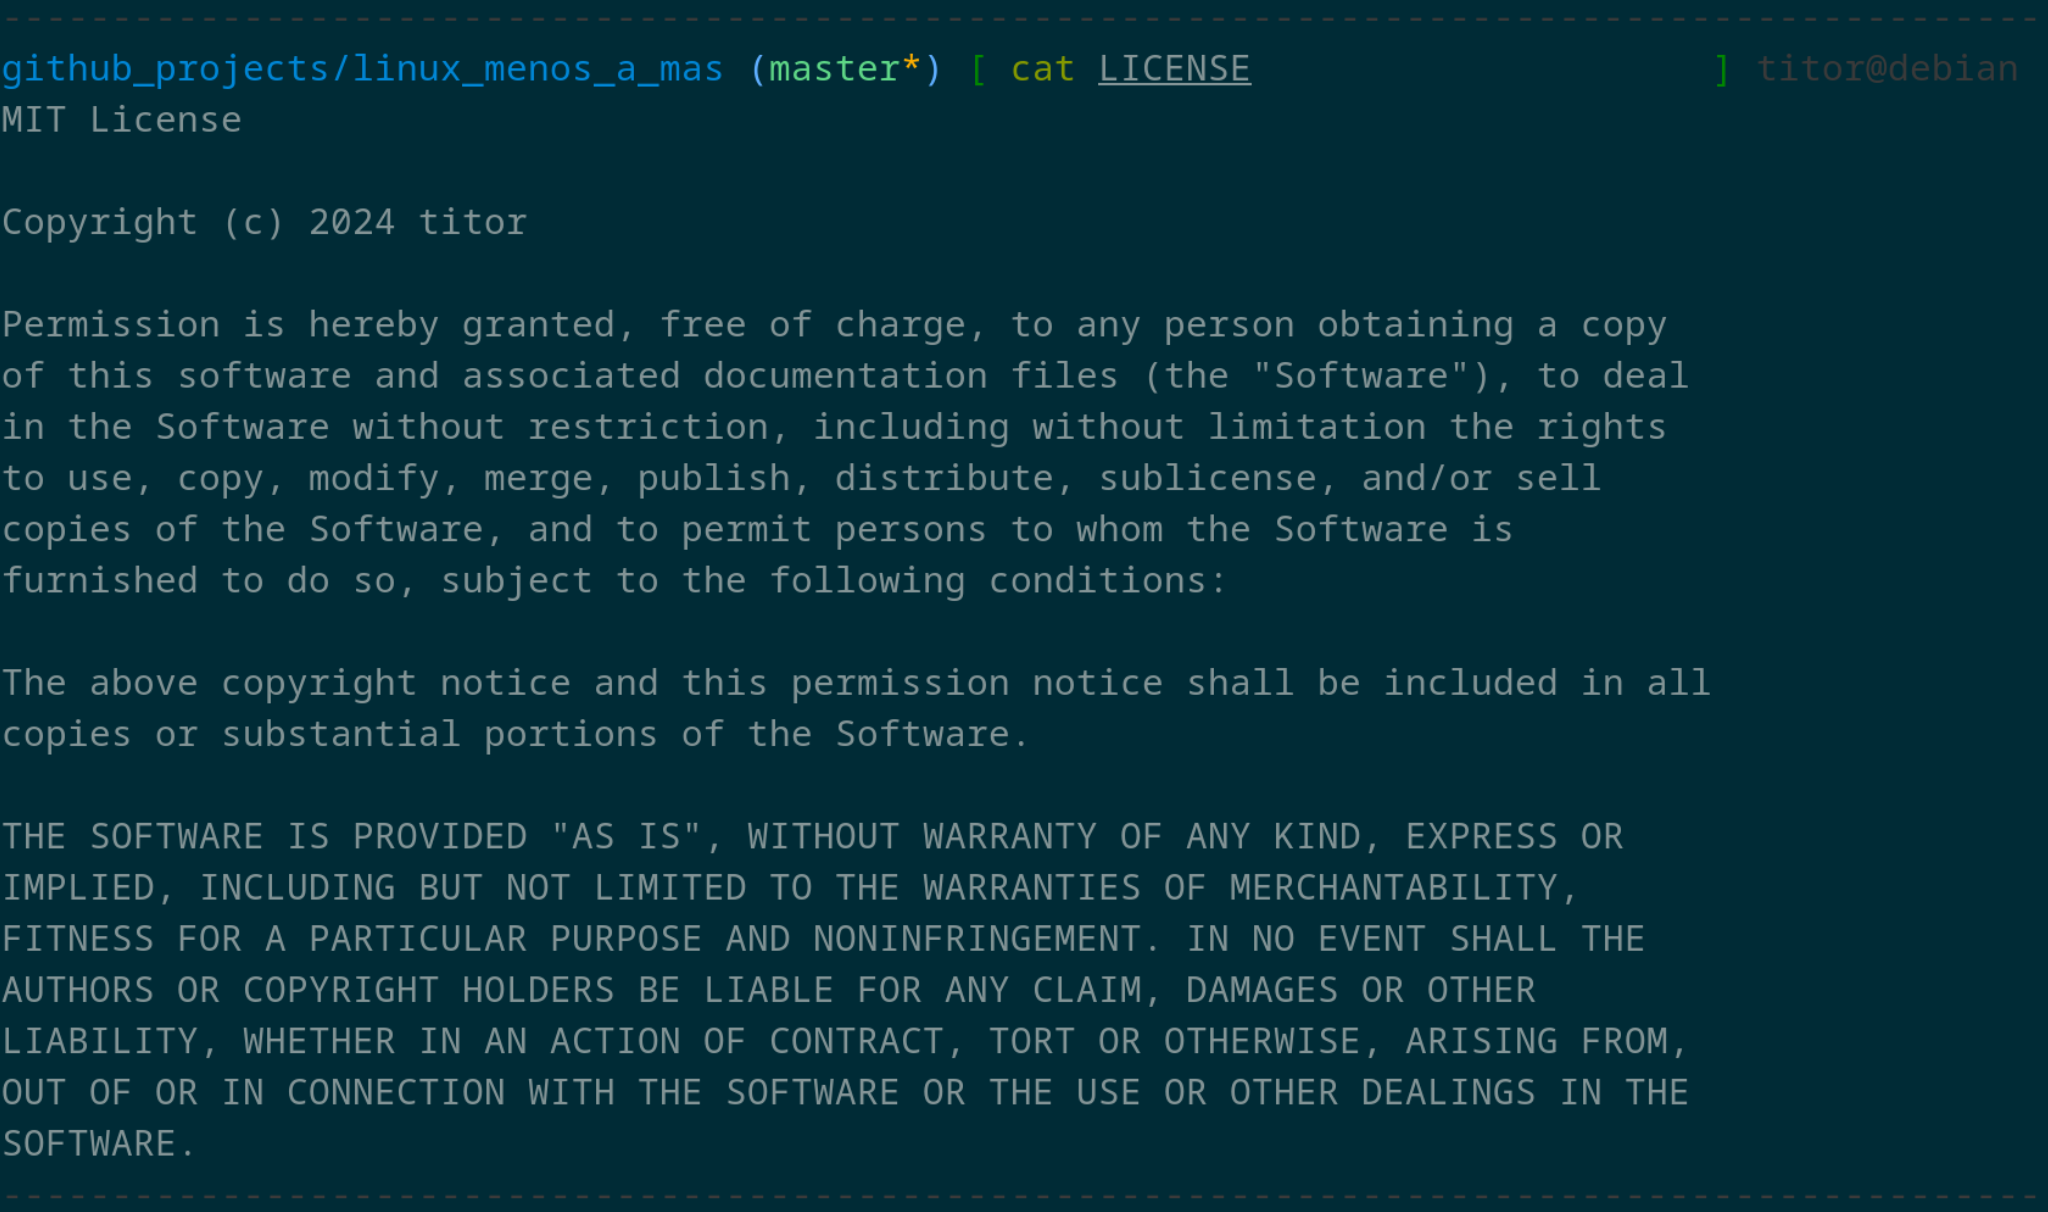
\includegraphics[width=1\textwidth]{image/chapter_01/cat_license.png}
	\caption{ejemplo cat.}
	\label{figura1}
\end{figure}

\begin{lstlisting}[language=bash]
\end{lstlisting}

\begin{lstlisting}[language=bash]
\end{lstlisting}
\end{enumerate}




